\documentclass[10pt, letterpaper]{article}
\usepackage[utf8]{inputenc}
\usepackage{hyperref}
\usepackage{graphicx}
\usepackage{url}
\usepackage[super]{nth}
\graphicspath{ {./assets/} }

\usepackage[margin=0.5in]{geometry}
\newcommand{\subsubsubsection}[1]{\paragraph{#1}\mbox{}\\}
\setcounter{secnumdepth}{4}
\setcounter{tocdepth}{4}
\newcommand{\tabitem}{~~\llap{\textbullet}~~}
\usepackage{makecell}

\begin{document}
\title{Terminus White Paper\\
    \large A digital voting system for the \nth{21} century}
\author{Vincenzo ``degli Abruzzi" Di Nicola \\ email \href{vincenzo@terminusfoundation.org}{vincenzo@terminusfoundation.org}
    \and Calogero Mandracchia \\ email \href{calogero@terminusfoundation.org}{calogero@terminusfoundation.org}
    \and Raffaele Nicodemo \\ email \href{raffaele@terminusfoundation.org}{raffaele@terminusfoundation.org}
} 
\date{June 10, 2019 \\ Draft v0.6}
\maketitle
\tableofcontents
\newpage

\section{Summary}
Voting is an action we perform in several different situations: some examples are song contests (e.g., Eurovision), reality shows (e.g., Big Brother), associations/councils (e.g., residents meeting), company’s decisions (e.g. shareholders meeting) or politics (e.g. country elections). 
Wherever allowed, digital voting systems have been introduced as tools to easen up voters to express their choice. However, most digital voting solutions in use nowadays are centralized and heavily affected by a number of problems: there is little assurance that the vote has been recorded correctly, or that the vote has not been modified later, or that voter anonymity is preserved.
\bigskip

On March 10, 2019, at Villaggio Rousseau in Milan we showcased the Proof of Concept of a digital voting system. The goal was to demonstrate that the above mentioned concerns can be drastically reduced, if not completely solved, by efficiently applying anonymous blockchain technologies to voting.
\bigskip

Some of the main assumptions and decisions our system is based on:
\begin{itemize}
\item A voting session has a start time and an end time. Once defined, it cannot be changed.
\item Each voting session is self-confined. That is, voting sessions are independent from each other, and share no data among them.
\item Here we assume the voter has his/her own digital identity. The way such digital identity is created beforehand is out of scope for the sake of this article: we are happy to discuss with digital identity solution providers about potential integrations in our system.
\item The whole End-to-End system must be completely \textbf{open source}. A voter must have no doubt that his/her vote has been cast anonymously and not tampered with.
\item Being open, external auditors - or even voters themselves - can verify that there was no malpractice (e.g. forgery) and the correctness of the results.
\end{itemize}

We will here describe how we came to our early stage design, and open up suggestions for further improvements.

\section{Voting categories}
From a general perspective, voting can be divided into two categories: “\textit{in loco}” voting (i.e., voter's physical attendance is required in defined locations to cast his/her vote) and remote voting (i.e., the voter can cast his/her vote from any location).\\ 
Within each category, different type of systems are used.
\begin{itemize}
\item \textit{In loco}
    \begin{itemize}
    \item Paper-based Voting Systems
    \item Hardware-based Voting Systems
    \end{itemize}
\item Remote
    \begin{itemize}
    \item Paper-based Voting Systems
    \item Digital Voting Systems
    \end{itemize}
\end{itemize}

The proposed solution deals with the latter of the categories above, i.e., Digital Voting Systems in a remote environment. This being said, it can be worthwhile to explore integrations with \textit{in loco} environments later in the future and improve current \textit{in loco} voting systems based on paper and/or hardware.

\section{Designing a remote digital voting system}
\subsection{Key features}
A remote digital voting system must be based on the following points:
\bigskip

\textbf{Immutability}
\begin{itemize}
\item Only the voter can add his/her vote. No one else can add votes.
\item No one can neither delete nor modify votes.
\end{itemize}
\bigskip

\textbf{Egality}
\begin{itemize}
\item Each vote must be equal to each other.
\item No voter can have his/her vote counted more than once.
\item Each voter must receive one and only one ballot.
\end{itemize}
\bigskip

\textbf{Anonymity}
\begin{itemize}
\item No one must know what a voter has voted for.
\end{itemize}
\bigskip

\textbf{Blindness}
\begin{itemize}
\item During the voting session, no one must know where the votes are going to. I.e., results must not be visible in real time.
\end{itemize}
\bigskip

\textbf{No forgery}
\begin{itemize}
\item Ballots cannot be forged, and their number must be exactly equal to the number of voters.
\end{itemize}
\bigskip

\textbf{Ad-hoc auditability}
\begin{itemize}
\item Provided that absolutely nothing is relinquished in terms of voter anonymity and result visibility, external auditors - or even voters themselves - must be able to verify that: 
\begin{itemize}
\item Number of ballots is exactly equal to the number of voters.
\item Each voter has received one and only one ballot.
\end{itemize}
\end{itemize}

\subsection{Technology}
We evaluated a number of different existing technologies. As described earlier, using centralized systems for digital voting has several weaknesses, some of which concerning vote recording, tampering of results and anonymity of voters. Furthermore, such systems are usually closed source (i.e., code not available to the public to analyze for possible issues) and under the operation of a single organization (which must be fully trusted upon).
\bigskip

On the other side, Blockchain technologies provide high levels of immutability, accessibility and reliability. That is why we believe that they are very suitable for digital voting systems.\\
At the same time, each Blockchain technology has its own peculiar strength. We discarded the two most famous ones (Bitcoin and Ethereum) since they are completely transparent: that is, anyone can see detailed transaction information on the Bitcoin and Ethereum Blockchains. This is not acceptable in a digital voting system: voting trends would be known in real time, and privacy of voters undermined at its very core.\\
That is the reason why we instead paid particular attention to two other Blockchain technologies: Zcash and Monero. They stand out for their strong focus on anonymity, which we believe to be of paramount importance and cannot be left as an afterthought. Such privacy-oriented Blockchain solutions, along with additional operational measures, can solve all the key points of a digital voting system.
\bigskip

\subsubsection{Blockchain network types}
From a network point of view, blockchain technologies may be divided into 2 areas:
\begin{itemize}
\item Permissionless blockchains (also called "public" blockchains)
\begin{itemize}
\item Bitcoin
\item Ethereum (public)
\end{itemize}
\item Permissioned blockchains (sometimes also called "private" \footnote{Quite an unlucky name collision. Private blockchains per se are not related with anonymity: "private" here means that not everyone is allowed to run a blockchain node} blockchains)
\begin{itemize}
\item Quorum (a permissioned version of Ethereum)
\item Hyperledger
\item Corda
\end{itemize}
\end{itemize}
Anyone can join and run a node in a Permissionless blockchains. This is undoubtedly a strong advantage, since the network is not run by any single entity (i.e., akin to a DB controlled by a single owner) but possibly a large variety of people. At a first sight, this seems the right solution for a remote e-voting system.
At the same time, a voting system must fulfil 2 operational requisites:
\begin{enumerate}
\item Voting recording time
\item Voting cost
\end{enumerate}
Currently, no permissionless blockchain can guarantee both requisites. Some known occurrences:
\begin{itemize}
\item Recording time: November and December 2017 saw a teardown of the Bitcoin network. Transactions remained unconfirmed for several days, if not eventually disappearing from the mempool~\cite{CCN:700M:11-Nov-2017:Online}.\\
A voting session must have a beginning and a defined end: having votes linger	unpredictability in a network, or any risk that they may disappear, undermines the vote system.
\item Cost: December 2017 saw the incredible popularity of CryptoKitties, a decentralized application based on Ethereum. This caused an unprecedented spike in transaction fees on the Ethereum network~\cite{HackerNoon:CryptoKitties:15-Dec-2017:Online}.\\
\end{itemize}
We are hopeful in future enhancements. For instance, Lightning Network~\cite{LightningNetwork:Online} technologies may address scalability issues and, as a result, confirmation times. Furthermore, sidechains such as Tari~\cite{Tari:Online} may allow to issue digital assets (e.g., vote tokens) at a fixed cost.
\bigskip

However, until these two points are addressed, it is tough to rely on permissionless blockchain for voting systems. At the same time, we are aware of the concerns regarding trust in a permissioned blockchain.\\
This is the reason why, for the time being, we opted for a \textbf{hybrid permissioned blockchain} solution. In such solution:
\begin{itemize}
\item Sealers are nodes run by pre-authorized separate entities, which can create ("seal") transaction blocks 
\begin{itemize}
\item In addition, by choosing anonymous blockchain technologies, such as Monero or Zcash, sealers cannot distinguish data in the underlying transactions, thus preventing a malicious sealer to effectively tamper the voting session.
\end{itemize}
\item Supporters are secondary nodes which can be run by everyone. They have access to the blockchain: cannot create blocks, but can watch them and be aware if something suspicious happens.
\item Rules could be put in place so that a subset of supporter nodes are eventually promoted to sealer nodes.
\begin{itemize}
\item This approach resembles the dynamics existing at the \textbf{United Nations Security Council}. A set of predetermined sealer nodes (akin to the UN Security Council 5 permanent members) and a set of supporter nodes that are temporarily promoted to sealer nodes (akin to the UN Security Council 10 non-permanent members).
\end{itemize}
\end{itemize}
\subsubsection{Zcash technology}
Zcash is one of the so-called anonymous cryptocurrencies. Its underlying technology is based on the Zero-Knowledge Proofs (ZKP): this is a sophisticated cryptographic method that allows "the prover" to prove to "the verifier" that a statement is true without revealing any additional information on the statement itself.\\
Zcash uses the zk-SNARK, a category of ZKP. Its main advantages are: no need for interaction between the prover and the verifier, and fast verification even for large statements.
\bigskip

The requirement for the use of zk-SNARK in Zcash is to have a common reference string shared, usually referred as the public parameters of the system. This is done in the beginning of the blockchain and is called the "Trusted Setup".\\
A malevolent user that created the trusted setup can hold the secret (called "toxic waste") used to generate the parameters; thus acquiring the power to produce infinite counterfeit coins.\\
To prevent such behavior, Zcash used the Multi-Party Computation Ceremony, where a small number of participants personally generates a piece of the secret. For the system to be successful, at least one person has to correctly destroy the toxic waste.
The ceremony is a very long and risky procedure: it involves using new devices, specific hardware modification, and live-proof recording. Videos explaining the full ceremony are available online~\cite{ZcashCeremony:YouTube}.
\bigskip

For a digital voting system, we feel the MPC Ceremony may not be the best approach, as well as the trusted setup concept. Therefore, we put Zcash aside.\\
Even though we did not choose zk-SNARKs, there is another variant of ZKP which requires no trusted setup: it is called Bulletproof. This is already been applied in Monero, making transactions considerably smaller in size, and we would like to experiment more on such technology.
\subsubsection{Why Monero technology}
We believe Monero is the most suitable technology for a digital and remote voting system. As a cryptocurrency, it has has proven its strength in highly adversarial environments: it has an extreme degree of privacy protection, and its community strives to increase it even further.
\bigskip

We are by far not the first ones to think that the technological prowess behind Monero can be applied to voting. We took inspiration from the CryptoNote protocol (on which Monero is based) that uses an optimized version of the Ring Signature scheme described by Eiichiro Fujisaki and Koutarou Suzuki~\cite{10.1007/978-3-540-71677-8_13}: the key application mentioned in the paper is actually anonymous voting.
\bigskip

We believe in \textbf{anonymity first}: this must be the main key pillar of any digital voting solution. It is important to stress that anonymity is native to the Monero protocol, and it is very well battle-tested. Other technologies, such as Bitcoin, try to achieve anonymity by adding second layers (e.g., Lightning Network); however, as of today, such incremental approaches do not provide the same guarantees as of native solutions.
\bigskip

Below a summary of the key features a digital voting solution must satisfy, along with their technical solutions. Roles (such as Administrator and Custodian) are described in the following section.

\begin{center}
  \begin{tabular}{ | l | l | }
    \hline
      Key feature & Solution \\ \hline
      \tabitem No external entity can add/remove/modify votes & Native to Blockchain technologies \\ \hline
      \tabitem No one must know what a voter has voted (anonymity) & Ring Signatures of voters \\ \hline
      \tabitem \makecell{No one must know where the votes are going to \\
                         (results must not be visible in real time)} & \makecell{Stealth address of vote receivers + vote receivers \\
            secret keys safe management by external Custodians} \\ \hline
      \tabitem \makecell{Ballots cannot be forged, and its number must be\\
         the same of voters} & Blockchain tokens generated before voting session begins \\ \hline
      \tabitem Each voter must receive one and only one ballot & \makecell{Blockchain tokens sent by the Administrator to voters\\
               before voting session begins} \\ \hline
      \tabitem \makecell{Auditor must be able to verify the 2 points\\
         above (number of ballots == number of voters; each voter \\
         has received one and only one ballot) without relinquishing \\
         anything in voter anonymity and vote visibility} & 
         \makecell{Auditor has access to voters view keys, thus verifying that \\
         Administrator has indeed sent one token to each voter} \\ \hline
      \tabitem No voter can have his/her vote counted more than once & Native to Blockchain technologies \\ \hline
      \tabitem Each vote must be equal to each other & Token fungibility \\ \hline
  \end{tabular}
\end{center}
\subsection{Roles in the system}
\begin{itemize}
\item \textbf{Voters}
\begin{itemize}
\item People who vote
\begin{itemize}
\item In a real-world paper voting analogy, Voters are akin to electors.
\end{itemize}
\end{itemize}
\item \textbf{Vote Receivers} (for ease of readability, also simply called "Receivers")
\begin{itemize}
\item Entities who receive the votes
\begin{itemize}
\item In a real-world paper voting analogy, Voters are akin to candidates.
\end{itemize}
\end{itemize}
\item \textbf{Administrator}
\begin{itemize}
\item Entity which, before voting session begins, grants one ballot to each Voter
\begin{itemize}
\item In a real-world paper voting analogy, Administrator is akin to poll clerks that give a ballot to each eligible voter.
\end{itemize}
\end{itemize}
\item \textbf{Auditor}
\begin{itemize}
\item Entity which ensures no foul play is done the Administrator
\begin{itemize}
\item {In a real-world paper voting analogy, Auditor is akin to scrutineers that ensure there is no malpractice.}
\item {Any Voter might also be an Auditor.}
\end{itemize}
\end{itemize}
\item \textbf{Custodians}
\begin{itemize}
\item Entities which, before voting session begins, create Receivers secret keys, publish Receivers public keys, but cannot show Receiver secret keys
\begin{itemize}
\item In a real-world paper voting analogy, Custodians are akin to militaries that protect the ballot box to be closed till the end.
\end{itemize}
\end{itemize}
\item Node
\begin{itemize}
\item \textbf{Sealers}
\begin{itemize}
\item Entities which run the underlying blockchain software solution and can create ("seal") blocks.
\begin{itemize}
\item In a real-world paper voting analogy, it is a combination of poll clerks and scrutineers that ensure no vote is added/deleted/modified during the voting session.
\item The reason why we added this Sealers role is explained in the section above. We hope that, through technological advancements, this role can disappear in the future.
\end{itemize}
\end{itemize}
\item \textbf{Supporters}
\begin{itemize}
\item Entities which run the underlying blockchain software solution but can only watch.
\end{itemize}
\end{itemize}
\end{itemize}

\section{Proof of Concept}
\subsection{Demonstration}
On March 10, 2019, at Villaggio Rousseau in Milan we showcased a simple Proof of Concept: voters were asked to pick one of four choices of food they would have liked to eat at the end of the event. Each of the food choices (pizza, apple, oranges, sweets) had a Vote Receiver wallet associated to them.
\bigskip

There was only one voting session, and at the end results were published. 
Had additional voting sessions been scheduled, the whole process would have been recreated from scratch (i.e., “one voting session, one blockchain”).

\subsection{Mobile application}
We forked what at the time was the stable version of Monerujo (v1.10.10): it is a Monero lightwallet developed by m2049r~\cite{Monerujo:Online}, and we are very grateful for its quality.
\bigskip

The v1.10.10 of Monerujo was still using the Monero v0.12; so first of all we had to replicate all updates done for the v0.13.0.4 in this version. We also introduced some custom graphical tweaks, and updated the seed node list. 
\subsection{Administrator dashboard}
For sake of this Proof of Concept, we created a dashboard where the Administrator could easily start and stop the voting session, and finally calculate results, without having to perform all the operations from the command line. 
\subsection{Blockchain technology}
We forked what at the time was the stable version of Monero (v0.13.0.4). As we already mentioned earlier, we believe Monero is the most suitable technology for a digital voting system, with an ambitious roadmap for future enhancements.
\bigskip

We removed all transaction fees (i.e., set to zero) and all their relative checks. We also introduced a few tweaks on the wallet side in order to allow vote transactions to be mined. Then we began with the system initialization.
\subsubsection{Before Voting Session}
Before starting the voting session, we had to configure the network. For demonstration purposes, we setup 5 instances on AWS: each instance ran a modified version of monerod (voting-chain daemon).\\
We did not modify the consensus protocol (except by removing the master nodes of the Levin protocol); at the same time, we wanted to achieve a sort of “artificial PoA”. We decided to keep things simple: we binded the daemon on localhost and linked directly everyone to everyone through SSH tunnels. At the end, we had a total of 20 tunnels (5 node * 4 connections), since SSH is unidirectional.
\bigskip

Once ready, all machines started mining at startup with same fixed-difficulty (100), and block rewards were sent to a special wallet called “miner”. This is a temporary solution just for demonstration, which will be removed with proper improvements (see later section [x]).
\bigskip

Our system uses one blockchain (or, in the future, one sidechain) for each voting session: this prevents people from using unspent vote tokens of a previous election to a new one. As a convention, 1 XMR equals to 1 vote token. If, by any chance, a “disturber” voter sends a fractional XMR token value to the Vote Receiver, such vote will not be counted at the end.
\bigskip

We also created an "Admin" wallet. N transaction (where N is the number of Voters) were sent by the “miner” wallet to the Admin wallet: each transaction had as amount 1 XMR. This was also useful to start the creation of Ring Signatures. In the improvement section [x] we discuss the best Ring Signature size and how to create a good number of available mixins.
\bigskip

At last, we set up the Vote Receivers. For sake of this Proof of Concept, the Administrator had access to a server where, through a simple dashboard, s/he could:
\begin{itemize}
\item Create Vote Receivers wallets
\item Start a voting session
\item Enable Voters
\item Stop a voting session
\item Calculate results
\end{itemize}
The Administrator kept locally all the Vote Receivers keys. Of course, this is not acceptable in a real-life voting system: the proper way to address Vote Receiver key management is discussed in later section [x] with the introduction of a custodial system.
\bigskip

For this demonstration, the Vote Receivers were: 
\begin{enumerate}
\item Pizza Margherita
\item Apple
\item Orange
\item Sweets
\end{enumerate}

\subsubsection{During Voting Session}
The voting session lasted 1 hour (from 10:00am to 11:00am). During such time, 67 attendees of Villaggio Rousseau volunteered to install and use on their Android phones an application, essentially a customized fork of “Monerujo”. 
\bigskip

Each attendee (“Voter”):
\begin{itemize}
\item Created a Voter wallet
\item Sent Voter wallet address to the Administrator
\item Received a vote token by the Administrator
\item Sent the vote token to one of the four Vote Receivers
\end{itemize}

\subsubsection{End of Voting Session and results}
At 11:00am on March 10, the Administrator stopped mining on each node, thus terminating the voting session.\\
Results were immediately announced by publishing the balance of each Vote Receiver wallet.
\bigskip

A total of 67 Voters took part to the 1-hour voting session demonstration. 53 of them actually cast a vote:
\begin{itemize}
\item Pizza Margherita - 30 votes
\item Orange - 12 votes 
\item Apple - 6 votes
\item Sweets - 5 votes
\end{itemize}
By the way the system has been design, there is no way of knowing who the 14 people who did not cast their vote were.
\bigskip

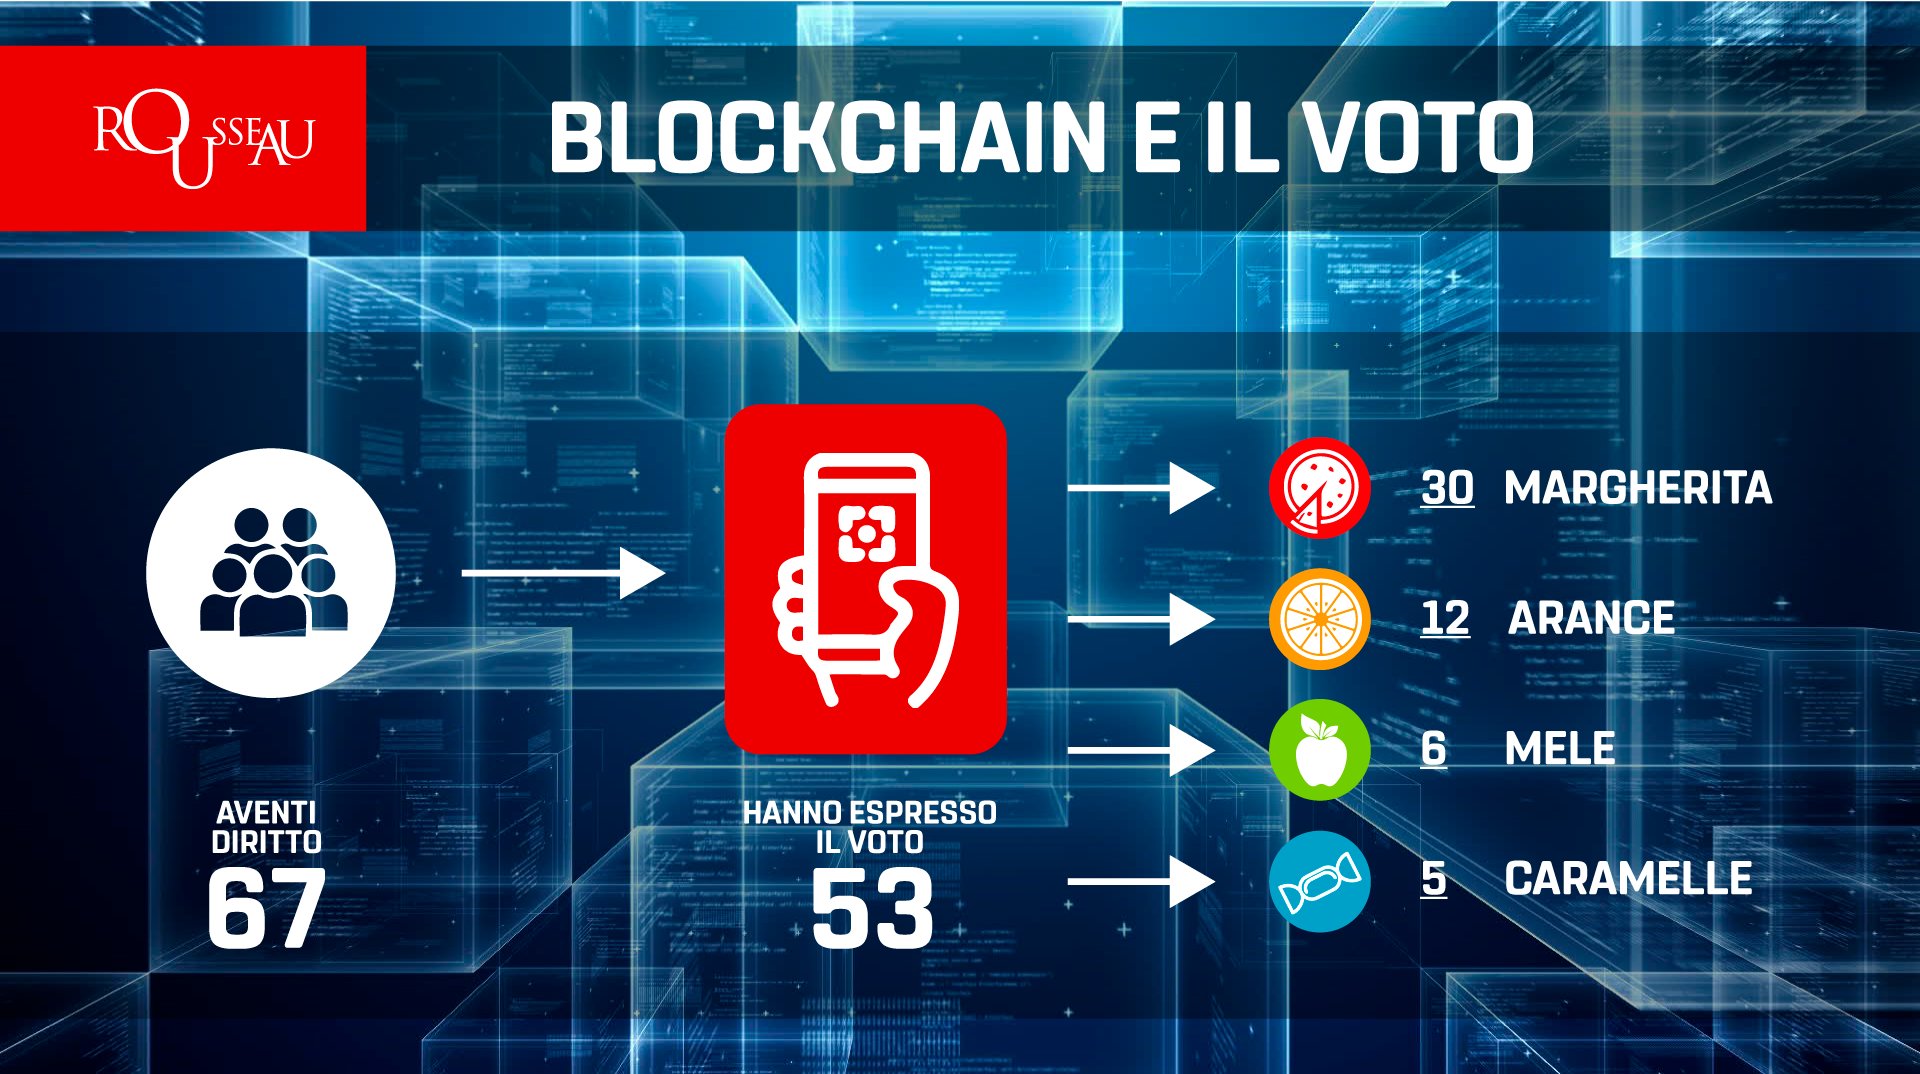
\includegraphics[width=0.8\textwidth]{blockchain_voto.png}

\section{Improvements}
The showcased Proof of Concept has obvious limitation and is just a starting point. Its real-life demonstration provided us with plenty of ideas and food for thoughts for future refinements. Below we describe some possible improvements.
\subsection{Block Reward}
In order to further guarantee that no additional vote tokens are created during a voting session,  block rewards must be zeroed out.\\
When monerod starts, a predetermined fixed number of tokens will be generated at the first block. Such number of tokens must be exactly equal to the number of Voters.
\subsection{Vote Receivers publishing}
The Proof of Concept relied on a server where the Voters can fetch information about Vote Receiver names and addresses. This is quite a vulnerability: an intruder may enter such a server, add/delete Vote Receivers or, worse, switch names with addresses (thus a Voter may think s/he cast his/her vote to Receiver A, while instead the vote went to Receiver B).
\bigskip

This can be easily fixed by removing such a server, and publishing in the real world the addresses of the vote receivers. During the voting session, each Voter must manually enter the address of the Vote Receiver. Alternatively, a more human-readable solution might involve OpenAlias~\cite{OpenAlias:Online}.

\subsection{Vote Receivers private keys custody}
Before the voting session begins, Vote Receivers private/public keypairs must be created.
This brings up a challenge. If a Vote Receiver has access to his/her private keys, s/he can see in real-time the voting session results. This cannot be allowed, since it would break one of the key aspects of a voting session (a Vote Receiver may leak results in real-time, or take advantage of this knowledge).\\
The showcased Proof of Concept brings an even greater concern, since it relies on a server where the Vote Receivers secret keys are created and stored.
\bigskip

All of this can be effectively solved by introducing the role of “Custodians”; that is, independent people in charge of protecting secrets.\\
Let’s consider N Custodians, and a safe environment where Vote Receiver private keys are created. These keys are then split into N shares using algorithms such as Shamir Secret Sharing, and a threshold of M (M <= N) is set. That is, it would require at least M Custodians to be able recreate the Vote Receivers private keys.\\
The corresponding Vote Receivers public keys are generated along with the private keys, and they can obviously be shared with the world so that Voters know where to send their transaction to.
\bigskip

\underline{Such custody schemes are today well used in the cryptocurrency world to protect wealth}: they involve safe procedures and hardware (e.g. HSM), which can be also directly applied in this case.
\bigskip

At the end of the voting session the blockchain is frozen: no more records can be added. At that point the voting count begins: Custodians would recompose the Vote Receivers private keys and calculate the balance of each Vote Receiver: that is, the number of votes received by each Vote Receiver.
\bigskip

After the voting session, Vote Receiver private keys are published by the Custodians to the world, so that everyone is able to verify the correctness of the results on the then-frozen blockchain.
\bigskip

Note: this solution relies on the concept of Custodians. If at least M Custodians collude, they might get access to Vote Receiver private keys and may even transfer votes from one Vote Receiver to another. However, if such a dishonest behavior happens, it will be easily noted by everyone once Vote Receiver private keys are published. 
\subsection{Consensus mechanism}
As we already mentioned earlier, for the sake of this Proof of Concept we did not modify the consensus mechanism. We binded the daemon of all 5 nodes on localhost and linked directly everyone to everyone through SSH tunnels.\\
For the future, we would like to introduce the concept of Sealers (pre-authorized separate entities allowed to create blocks) and Supporters (secondary nodes which can be run by everyone, and able to watch blocks and transactions). In this scenario, while waiting for scalable solutions like sidechains, we need to develop and introduce a Proof of Authority mechanism as has already been done by:
\begin{itemize}
\item Blockstream
\begin{itemize}
\item Used in Elements platform
\end{itemize}
\item Ethereum
\begin{itemize}
\item Used in the Rinkeby and Kovan testnet to protect against spam attack
\end{itemize}
\item Quorum
\begin{itemize}
\item Used in the JP Morgan coin
\end{itemize}
\item VeChain
\begin{itemize}
\item Used natively
\end{itemize}
\end{itemize}

Sealers, the "authority nodes", are independent entities which must not belong to the same organization and are interested to keep the network up and running. In order to ensure a further degree of independence, we suggest a “\textit{United Nations Security Council}”-inspired mechanism (which has 5 permanent members and 10 rotating non-permanent members). That is, in our proposal a Supporter node may be promoted to a Sealer node on a temporary basis.
\bigskip

Furthermore, thanks to Monero features, no node will not be able to understand the voting session underlying data, and everyone who joins the network as “supporter” node will be able to determine if sealers act maliciously.
\bigskip

From a technical point of view, there are two main approaches that could be used:
\begin{itemize}
\item Signers Blocks: implemented by Blockstream in Elements project, consist of identified nodes who are the only ones allowed to sign and create blocks with their private keys.
\item Authority Masternode: based on Proof of Stake consensus, implemented among others by VeChain.
\end{itemize}

\subsection{Voting session termination}
The voting session duration must be known, and cannot be extended. Let’s say 12 hours.
If the system creates blocks every, say, 10 seconds, then the last block that the voting session must be block number 4,319. The sealers won’t mine any block greater or equal to number 4,320.

\subsection{Blockchain freezing}
At the end of the voting session, the Administrator and/or Auditors can hash (e.g. SHA-256) the blockchain and “notarize” it on one or more public blockchains. As an example, the blockchain hash can be saved in the OP\_RETURN field of a Bitcoin transaction.\\
If needed, this notarization operation can be done not only at the end of the voting session, but even several times during the voting session.
\subsection{Voter anonymity}
Ring Signatures (RS) are one of the most important aspects in Monero: they preserve privacy and untraceability, two required features of an anonymous ecosystem such a Voting System. 
\bigskip

We are waiting for anonymous digital assets to be effectively implemented on the public Monero network (e.g. Tari). Until then, our approach requires to create a new Blockchain for each voting session; therefore, we must pay great attention to the quantity and quality of mixins, and prevent external chainalytics entities from being successful in de-anonymizing (even partially) data. 
\bigskip

An initial setup phase in our system is needed in order to have enough TXOs to properly create RS. Starting from block number 1685555, Monero has had a fixed size of 11 mixin for each RS; if needed, we could increase this size to improve Voters privacy. 
\bigskip

Other techniques could be implemented to improve the mixins quality, with the idea that the greater the number of transactions the more secure the network is:
\begin{itemize}
\item Using a 2-phase approach: each Voter, before sending the vote token to a Vote Receiver, makes a first transaction to a new wallet created by him/her, and then from this new address casts the vote to the chosen Vote Receiver. Of course, all this process will be invisible for a simple user and completely automatized in the application.
\begin{itemize}
\item This could be hard to this system (or impossibile) to implement if we choose to have different types of addresses (see discussion in section below) and allow Voters to send transaction only to Vote Receiver addresses.
\end{itemize}
\item Creating fake transactions with zero amount: To increase the number of transactions, thanks to the Ring Signature Confidential Transaction feature natively available in Monero, it is not possible for an external chainalytics entity to understand or calculate transactions amount: only senders and receivers can do it. This means that, if we allow the Administrator to create fake transaction towards fake Vote Receiver addresses with no amount, no-one will be able to understand that transaction is vote-related or not. 
\item Mixin selection: the mixins selection should ensure that every TXO appears in at least 2 (or more) RS. This way it would more challenging to analyze whether a TXO was spent or not.
\end{itemize}
\subsubsection{Quality of decoys}
The selection of decoys (mixins) used the form a Ring Signature is handled by the Voter’s wallet. Two questions arise from this:
\begin{itemize}
\item Is the algorithm being currently used by Monero suitable for this proposed voting system?
\begin{itemize}
\item All happens in over a short fixed period of time: can this give sensitive intel about who the voter is?
\end{itemize}
\item Whichever algorithm is chosen, can we really rely on the wallet? 
\begin{itemize}
\item This is a critical question. A briber may build a corrupted version of the wallet, force the Voter to use it, and de facto deanonymize the Voter.
\end{itemize}
\end{itemize}

To address these issues, enforcements must be done at protocol level instead of client level. That is, the client must not be able to randomly choose the decoys, but follow certain rules: else, the protocol will reject the transaction. This has to be done in a provable deterministic way, still without weakening Ring Signatures properties. We may add some requirements on how the decoys must be chosen: for example, for a TXO (given by the Administrator to the Voter at block number 15) the wallet may include in its ring only decoys that are in the same block (number 15) or in its immediate adjacency. The network can verify this quite easily and reject transactions that do not follow this requirement. Further analysis is needed for this approach, in order to be sure that the Administrator’s knowledge of TXOs distribution does not impair Voters anonymity.\\
Another, though more sophisticated approach is to use keyed hash functions, as described in Chator and Green’s paper~\cite{8406559}. This allows to efficiently increase the RS size, and can be applied to improve the overall quality of decoys.

\subsection{Node communication improvement}
In order to remove any sort of traceability, the Voter application must communicate with more than one remote node. Were it to communicate with only one remote node, the remote node would know the TXOs asked by the Voter for its mixin: when the Voter application sends its TXOs for the ring to the same remote node, the remote node might guess which the real transaction TXO is. 
\bigskip

Tracing attacks through malicious remote nodes are well known: for example, by sending fake errors to wallets. At the same time, in an open network like the one we are designing, everyone may run his/her own Supporter node. This solves concerns of sending transaction to a malicious remote node.
\bigskip

At the same time, in an open network like the one we are designing, everyone may run his/her own Supporter node. This solves concerns of sending transaction to a malicious remote node.
\subsection{Vote delegation}
This can be a desidered feature, or not. In the current Proof of Concept, a Voter may actually send his/her vote to a fellow Voter: the mobile application does not have such an option, but of course it is easy to customize the mobile application and allow it. Of course, an Auditor (that has access to private view keys) will be able to see that a given Voter has received more than one token, and raise a warning if such a behavior is not allowed; yet, this cannot prevent the Voter to cast his/her multiple delegated votes.
\bigskip

If vote delegation is not allowed, then the solution must address such an issue. This may be solved by creating different set of addresses: one set for Voters, one set for Vote Receivers, one set for the Administrator. Administrator can only send tokens to Voters (beginning of voting session), and most importantly Voters can only send tokens to Vote Receivers. Illicit transactions must not be recorded on the blockchain.
\subsubsection{Different type of addresses}
Specific addresses and transactions can be created in order to prevent vote malpractices. Administrator, Voters and Receivers can be identified by different set of addresses (similar to the differences between mainnet and stagenet).\\
Each address type will have different permissions:
\begin{itemize}
\item Administrator address
\begin{itemize}
\item Cannot receive transactions from Voters or Vote Receivers
\item Can send transactions only to Voter addresses
\end{itemize}
\item Voter address
\begin{itemize}
\item Can receive transaction only from Administrator addresses
\item Can send transactions only to Vote Receiver addresses
\end{itemize}
\item Vote Receiver address
\begin{itemize}
\item Can receive transactions only from Voters addresses
\item Cannot send transactions
\end{itemize}
\end{itemize}

This can be useful to: 
\begin{itemize}
\item Prevent Voters to send his/her vote to other Voters
\begin{itemize}
\item Thus avoiding vote delegation 
\end{itemize}
\item Prevent someone to send Vote Receiver’s votes to another one
\item Prevent Administrator to send votes directly to Vote Receivers
\begin{itemize}
\item Of course Administrator could create fake Voters, recharge them and cast a vote to a Vote Receiver. Though, Auditors will be able to check that addresses recharged from Administrator are related to real Voters
\end{itemize}
\end{itemize}
\subsection{I2P-zero}
Some sensitive information (e.g., Voter IP address) may be leaked at the network level when making a transaction.\\
To mitigate such concern, Tor could be used. However, Tor relies on semi-trusted directory authorities, which determine who is allowed to relay traffic on the Tor network. This may be a major weakness.\\
VPN is another choice, but it also suffers from correlation attacks. It may be easy for large attacks to de-anonymize traffic.
\bigskip

In Monero this privacy leak was initially addressed with Kovri, but the project seems to have come to a halt. Recently the I2P-zero project~\cite{i2p-zero:Online} has been released: a standalone version of I2P with no dependencies, providing free and decentralized anonymity. It creates a private overlay network across the globe by using encryption and garlic routing techniques. This layer allows users to hide their geographical location and IP address.
\bigskip

Right now, with a major effort, in our solution it might be possible to trace back the route of a vote. This would leak the IP of the Voter who signed the ring: that’s why we would love to add I2P-zero as another tool to further anonymize the Voters.

\subsection{Proof that Vote has been recorded correctly}
Upon the Voter sends his/her vote, s/he has access to the following information:
\begin{itemize}
\item Vote Receiver address (of course)
\item Transaction id
\item Transaction key
\end{itemize}
With these information, the Voter can query the blockchain and be sure that:
\begin{itemize}
\item Vote has been recorded
\item Vote has been sent to to chosen Vote Receiver
\end{itemize}

While this provides the Voter with a complete guarantee that his/her vote has been recorded and will be counted correctly, it also opens a scenario where:
\begin{itemize}
\item An honest Voter is forced to vote for a Vote Receiver (e.g. under coercion or threat)
\item A dishonest Voter sells his/her vote to a briber
\end{itemize}

In both cases, the Voter may prove the coercer or briber that s/he complied. Such a situation happens all the time in the real-world: it’s extremely easy with remote paper voting, or even with in loco voting through pictures taken during the vote.\\
No voting solution (neither in loco nor remote) can prevent it. However, mitigations can be here put in place.
\subsubsection{Vote Invalidation}
A Voter may be enticed to sell his/her vote to a briber: the briber wants to be sure that the Voter has voted for Vote Receiver A, and wants proof. As mentioned above, the Voter can prove it by showing the briber the tuple “Vote Receiver A address, Transaction id and Transaction key”. Let’s assume though the the Voter is able to invalide his/her bribed vote: this will make the very concept of bribery a moot point.
\bigskip

In real-world, this is akin to a situation where the Voter marks the vote for someone on paper, takes a picture of the vote, shows such a picture to the briber (thus “proving” Voter has voted for the choice asked by the briber), but then the Voter completely taints the ballot thus making it invalid.

\subsubsubsection{Initial idea}
Let’s make a step back, and have the system require that each transaction must have a properly formed data in the “Transaction extra” field. Such data must also be encrypted with an “invalidation” public key known to the Voter. The corresponding invalidation private key must be kept by Custodians, and never revealed. \\
Let’s consider this flow:
\begin{itemize}
\item Voter (been bribed) send his/her Token to Vote Receiver A.
\item Voter (who instead wants to doublecross the briber) in this transaction populates the “Transaction extra” field with a special message stating that s/he actually wants this transaction to be invalidated.
\begin{itemize}
\item “Transaction extra” field data is encrypted with the invalidation public key, but no one (except for the Custodians) can decrypt it. 
\end{itemize}
\item Voter can prove the briber that s/he voted for Vote Receiver A, providing the tuple “Vote Receiver A address, Transaction id and Transaction key”.
\begin{itemize}
\item All seems good for the briber.
\end{itemize}
\item When the voting session is over, the count phase will take into account the special message in the “Transaction extra” field.
\begin{itemize}
\item By decrypting the content on “Transaction extra” and after its legit content verification, the Custodian and Auditor can know that Vote Receiver A count must be decreased by 1, thus effectively invalidating the vote.
\end{itemize}
\end{itemize}
This approach has one weakness. The briber may impose the Voter to enter a briber-predetermined data in “Transaction extra” (thus preventing the Voter to have an invalidating message), that the briber can actually verify.\\
However, a strong mitigation can be introduced. In order for the vote to be considered valid when counted at the end, the data in “Transaction extra” must have a reference a previous block hash (say, any of the previous 10 block hashes). This prevents the briber to have predetermined data in “Transaction extra” to give the Voter, and makes bribery much more challenging.
\bigskip

Though, by introducing a “time” variable into the voting system, the downside is that an honest Voter cannot be 100\% sure whether his/her vote has been counted. The Voter may casts his/her vote, but due to a network hiccup/congestion the transaction is recorded in the blockchain with a delay: if the “Transaction extra” data references, say, a block hash older than 10 blocks, then the vote would be considered invalid.
\bigskip

\subsubsubsection{Improved idea}
The blockchain solution discussed so far is based on the basis “1 Voter, 1 token”: once the token has been sent from the Voter to the Vote Receiver, it’s impossible to claim it back. So, at a first sight, allowing the Voter to invalidate his/her vote (without approaches like “Transaction extra” discussed above) seems unfeasible.
\bigskip

This might be solved if the Voter, when the voting session begins, receives from the Administrator 1 “vote” Token (as before) AND an additional “invalidation” Token (as technical amount, say equivalent to 0.0001 XMR of the vote Token). That is, let’s introduce a way to distinguish between tokens based on their underlying amount.\\
The process is the following:
\begin{itemize}
\item Voter (under coercion or been bribed) send his/her 1 vote Token to Vote Receiver A.
\item Voter (under coercion or been bribed) can prove the coercer/briber that s/he vote for Vote Receiver A, providing the tuple “Vote Receiver A address, Transaction id and Transaction key”.
\begin{itemize}
\item All seems good for the coercer/briber.
\end{itemize}
\item Voter can make a second transaction, using the additional 0.0001 invalidation Token.
\begin{itemize}
\item The “Transaction extra” field of the transaction is populated with the tuple “Vote Receiver A address, Transaction id and Transaction key”.
\begin{itemize}
\item I.e., the Voter is here proving that s/he sent an earlier vote to Vote Receiver A, but instead wants now this vote NOT to be counted.
\item The content of the “Transaction extra” field in encrypted using a an invalidation public key (only Custodians have access to the invalidation private key, and never disclose it to the public).
\end{itemize}
\end{itemize}
\item The coercer/briber has no clue that Voter has sent a second transaction, effectively asking the final vote counters to invalidate the vote (i.e. decrementing by one the total number of votes for Vote Receiver A).
\begin{itemize}
\item Decrypting the content on “Transaction extra” and after its legit content verification, the Custodian and Auditor can know that Vote Receiver A count must be decreased by 1 (in the pool of the 1 Token received).
\end{itemize}
\end{itemize}
Note:
\begin{itemize}
\item If the fractional Token transaction stands out because of its size (due to “Transaction extra”) and may damage Voter anonymity, then we may simply decide to have a properly padded “Transaction extra” data in every single transaction.
\end{itemize}
In conclusion, this approach adds a bit of complexity to the solution and the final vote count. However, it effectively allows a Voter to invalidate a vote previously cast, thus making bribery much less powerful.
\bigskip

Of course, being the invalidation “embedded” in the vote transaction, this solution does not solve the case where a Voter is under strict observation over the entire voting session and is forced to vote for a certain Vote Receiver.
\subsubsubsection{Further steps}
The idea described above effectively allows a Voter to invalidate his/her previous vote. What if, instead of simply invalidating it, the Voter may actually get a chance to vote again?
This would introduce the concept of private Smart Contracts (apparently been recently introduced by Dero~\cite{Dero:Online} - much further analysis is required).
\bigskip

Here’s a high-level view:
\begin{itemize}
\item Voter sends his/her vote token to Vote Receiver A
\item Voter changes idea. S/he send his/her invalidation token to a known Smart Contract
\item Upon proper validation, the Smart Contract does the following 2 actions:
\begin{itemize}
\item Sends the invalidation token to Vote Receiver A
\begin{itemize}
\item This tells Custodians and Auditor to decrease by 1 the number of votes of Vote Receiver A
\end{itemize}
\item Sends a new vote token to the Voter
\begin{itemize}
\item Within the invalidation token data, there must also be the address (or subaddress) of the Voter, so that the Smart Contract knows where to send the new vote token to
\end{itemize}
\end{itemize}
\item Voter can now vote again
\end{itemize}

By allowing a Voter to vote multiple times in a voting session, coercion/bribery concerns are drastically reduced. Of course, the approach here mentioned must be evaluated in details, and be sure that it is actually feasible and that Voter anonymity is indeed preserved.
\subsubsection{Receipt-freeness}
“Receipt-freeness” is a different approach to deal against bribery. As also discussed before, a Voter may be enticed to sell his/her vote to a briber: the briber wants to be sure that the Voter has voted for Vote Receiver A, and wants proof. Let’s assume that the Voter complies but, even so, the briber can still not be sure that the Voter actually did vote for Vote Receiver A. If such a solution is implemented, then bribery effectively becomes useless.
\bigskip

To describe this situation more in details, let’s say a briber reaches out to a Voter and asks him/her to vote for Vote Receiver A. Let’s say though that the Voter instead honestly votes for Vote Receiver B, thus getting the resulting voting tuple “Vote Receiver B address, Transaction id and Transaction key”. If the Voter is able to transform his/her resulting voting tuple into a new seemingly-legit tuple “Vote Receiver A address, Transaction id new and Transaction key new” to be given to the briber, then the briber would think that the Voter voted for Vote Receiver A (and the bribery was successful) even though this is not true.
\bigskip

This approach require further investigation, and may require proper set up. For example, before the Voting session begins, the Administrator might cast one vote towards each Vote Receiver and publish the resulting voting tuples: this extra information could allow the Voters to successfully transform their resulting voting tuple.
\section{Conclusion}
We have here described a system that, with the proper enhancements, it proves to be superior to the remote voting solutions used today. Voter anonymity, no forgery/stealing of ballots, no tampering of votes, and full verifiability of results. "\textbf{Don’t trust, verify}" is the principle we followed: an End-to-End open source system that can allow anyone to audit, have real-time visibility of the blockchain, and be certain of the correctness of the results. All of this, at a fraction of the costs of current remote voting solutions.\\
As also happens in the real world, dishonest voters may decide to sell their vote: this is an unfortunate occurrence that happens in every system, be it based on paper or digital. In the proposed improvements we introduced ideas to allow a Voter to invalidate his/her vote, or vote again. Further research is needed: if successful, this will drastically reduce the effectiveness of a bribe.\\
We also want to stress that our system is based on the concept of “digital identities”: the way they are created is not addressed here, and we are interested in integration with appropriate technologies. For example, biometrics controls can assure that the person is indeed real and present, and can be added on top of the voting system.\\
Finally, we believe that our solution may in the future play a role not only in remote voting, but also in “\textit{in loco}” voting. If there are concerns such as threat/coercion, voting sessions can be done inside classic booths: instead of paper/pencil, there would be a customized on-premise version of this system. This would effectively combine the best of both worlds, reinforcing their strengths and removing concerns of frauds. Of course, this is looking far ahead in the future: it is a suggestion that would require very thorough experimentation.\\
Our main and only focus has been on addressing the several limitations and issues of the remote voting systems that are being used nowadays. We believe that, wherever remote voting systems are allowed, anonymous blockchain-based solutions like ours are the appropriate choices. There is no longer a need to trust anyone: voters’ participation and their contribution to the decision making of their communities is likely to increase.
\section{Credits}
\textbf{In progress}

\bibliographystyle{unsrt}
\bibliography{references}
\end{document}
